\section{1 de febrero de 2021}

\begin{definition}
\begin{itemize}
    \item Bola abierta $Br(a)=\{x\in M\ni d(x,a)<r\},\quad r>0$
    \item Abierto: $Br()$ o $\bigcup,\bigcap$
    \item Vecindad $x$ abierta: $A\ni A$
\end{itemize}
\end{definition}

\begin{proposition}
$A$ es cerrado ssi $A'\subset A$\marginnote{Un conjunto es cerrado ssi contiene a sus puntos de acumulación.}
\end{proposition}
\begin{proof}
\begin{itemize}
    \item ($\to$)\marginnote{A probar: $A'\subset A\Longleftrightarrow$ si $x\in A'\implies x\in A\Longleftrightarrow $ si $x\not\in A\implies x\not\in A'$} Sea $A$ cerrado y sea $p\not\in A\implies p\in A^c$, pero $A^c$ es un abierto $\ni p\in A^c$ y $A\cup A^c=\emptyset\implies p\in\not A'\implies A\implies A'\subset A$
    \item ($\gets$) A probar: $A'\subset A\implies A$ es cerrado ($\Longleftrightarrow A^c$ es abierto). Suponga que $A'\subset A$ 
    y sea $p\in A^c\implies p\not\in A'\implies \exists G$, abierto, tal que: $p\in G$ y $$(G-\{p\})\cap A=\emptyset$$
    Como $p\not\in A\implies G\cap A=\emptyset\implies G\subset A^c$. Entonces si $p\in A^c\exists $ abierto $G\ni p\in G\subset A^c\implies A^c$ es abierto. 
    \begin{center}
        

\tikzset{every picture/.style={line width=0.75pt}} %set default line width to 0.75pt        

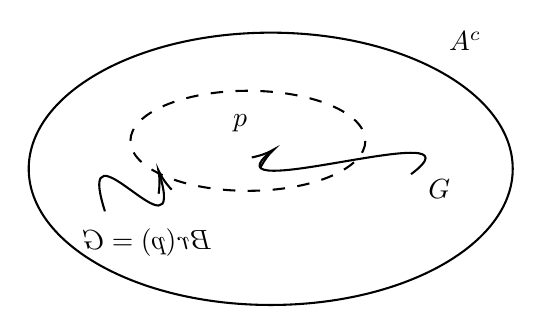
\begin{tikzpicture}[x=0.75pt,y=0.75pt,yscale=-1,xscale=1]
%uncomment if require: \path (0,300); %set diagram left start at 0, and has height of 300

%Shape: Ellipse [id:dp37154978089883683] 
\draw   (100,111.6) .. controls (100,75.37) and (152.2,46) .. (216.6,46) .. controls (281,46) and (333.2,75.37) .. (333.2,111.6) .. controls (333.2,147.83) and (281,177.2) .. (216.6,177.2) .. controls (152.2,177.2) and (100,147.83) .. (100,111.6) -- cycle ;
%Shape: Ellipse [id:dp6206196527695439] 
\draw  [dash pattern={on 4.5pt off 4.5pt}] (149,98.1) .. controls (149,84.79) and (174.34,74) .. (205.6,74) .. controls (236.86,74) and (262.2,84.79) .. (262.2,98.1) .. controls (262.2,111.41) and (236.86,122.2) .. (205.6,122.2) .. controls (174.34,122.2) and (149,111.41) .. (149,98.1) -- cycle ;
%Curve Lines [id:da7080138380886729] 
\draw    (284.2,114.2) .. controls (323.8,84.5) and (181.1,131.25) .. (217.06,103.08) ;
\draw [shift={(218.2,102.2)}, rotate = 503.13] [color={rgb, 255:red, 0; green, 0; blue, 0 }  ][line width=0.75]    (10.93,-3.29) .. controls (6.95,-1.4) and (3.31,-0.3) .. (0,0) .. controls (3.31,0.3) and (6.95,1.4) .. (10.93,3.29)   ;
%Curve Lines [id:da88098585793335] 
\draw    (136.71,132.07) .. controls (121.26,82.89) and (176.93,160.3) .. (162.9,113.65) ;
\draw [shift={(162.45,112.2)}, rotate = 432.56] [color={rgb, 255:red, 0; green, 0; blue, 0 }  ][line width=0.75]    (10.93,-3.29) .. controls (6.95,-1.4) and (3.31,-0.3) .. (0,0) .. controls (3.31,0.3) and (6.95,1.4) .. (10.93,3.29)   ;

% Text Node
\draw (301,44.1) node [anchor=north west][inner sep=0.75pt]    {$A^{c}$};
% Text Node
\draw (197,84.1) node [anchor=north west][inner sep=0.75pt]    {$p$};
% Text Node
\draw (291,115.1) node [anchor=north west][inner sep=0.75pt]    {$G$};
% Text Node
\draw (124.32,138.74) node [anchor=north east][inner sep=0.75pt]  [xscale=-1]  {$Br( p) =G$};


\end{tikzpicture}
    \end{center}
\end{itemize}
\end{proof}

\begin{proposition}
Si $F$ es un superconjunto cerrado de cualquier conjunto $A$, entonces $A'\subset F$ 
\end{proposition}
\begin{proof}
Sabemos que $F$ es cerrado y $A\subset F$. Como $A\subset F\implies A'\subset F'$. Como $F$ es cerrado, entonces $F'\subset F\implies A'\subset F$
\end{proof}

\begin{proposition}
$A\cup A'$ es cerrado. 
\end{proposition}
\begin{proof}

Se asume que $A^{\prime}$ que significa el conjunto de elementos limitantes con $A$. Para un conjunto $B$, Se denota cl $(B)$ como cerradura.
Desde que $\operatorname{cl}\left(A \cup A^{\prime}\right) \supseteq \operatorname{cl}(A) \supseteq A^{\prime},$ miramos
$$
A \cup A^{\prime} \subseteq \operatorname{cl}\left(A \cup A^{\prime}\right)
$$
entonces, se necesita probar que $A \cup A^{\prime}$ es cerrado.
Suponemos $x$ es un punto límite de $A \cup A^{\prime} .$ Si $x \in A,$ entonces no hay nada que probar, entonces suponemos $x \notin A$. Decimos que $U$ es un vecindario de $x$; entonces existe $y \in A \cup A^{\prime}, y \neq x,$ con $y \in A \cup A^{\prime} .$ Si $y \in A,$ entonces está comprobado. De otra forma $y \in A^{\prime} \backslash A$; si tomamos un vecindario $V$ de $y, V \subseteq U$; entonces hay $z \in A \cap V$, $z \neq y ;$ por lo que $z \in A \cap U, z \neq x$
\end{proof}

\begin{proposition}
$\Bar{A}=A\cup A'$
\end{proposition}
\begin{proof}
\begin{itemize}
    \item ($\supseteq$) Sabemos que $A\subset \Bar{A}$.\marginnote{$A\subset B\implies A'\subset B'$} Por otra parte, $\implies  A'\subset(\Bar{A})'\implies \Bar{A}\implies A'\subset \Bar{A}\implies A\cup A'\subset \Bar{A}$.
    \item ($\subseteq$) A probar: $\Bar{A}\subset A\cup A'$. Entonces, $A\subset A\cup A'\implies A\subset \Bar{A}\subset A\cup A'$
\end{itemize}
\end{proof}

\begin{proposition}
Si $A\subset B\implies \Bar{A}\subset \Bar{B}$
\end{proposition}

\begin{proof}
Si $A\subset B\implies A'\subset B'\implies A\cup B'\subset B\cup B'\implies \Bar{A}\subset \Bar{B}$
\end{proof}

\begin{proposition}
$\overline{A\cup B}=\Bar{A}\cup \Bar{B}$
\end{proposition}

\begin{proof}
\begin{itemize}
    \item $(\subseteq)$ A probar $\overline{A\cup B}\subset \Bar{A}\cup \Bar{B}$. Sabemos que $A\subset \Bar{A}$ y $B\subset \Bar{B}\implies A\cup B\subset \Bar{A}\cup \Bar{B}\implies A\cup B\subset \overline{A\cup B}\subset \Bar{A}\cup \Bar{B}$
    \item $A\subset A\cup B \implies \Bar{A}\subset \overline{A\cup B}$\\
          $B\subset A\cup B \implies \Bar{B}\subset \overline{A\cup B}$\\
          $\implies \Bar{A}\cup\Bar{B}\subset \overline{A\cup B}\cup \overline{A\cup B}\implies \Bar{A}\cup \Bar{B}\subset \overline{A\cup B}$
\end{itemize}
\end{proof}

\begin{remark}[Axiomas de Kuratowski]
\marginnote{Propone: Construir una topología de cerrados a partir de $k_1-k_4$}
\begin{itemize}
    \item $K_1$ : $\Bar{\emptyset}=\emptyset$
    \item $K_2$ : $A\subset\Bar{A}$
    \item $K_3$ : $\Bar{\Bar{A}}=\Bar{A}$
    \item $K_4$ : $\overline{A\cup B}=\Bar{A}\cup \Bar{B}$
    \end{itemize}
\end{remark}

\begin{definition}
$$\frac{f(A)}{f(C)}$$
\begin{center}
    

\tikzset{every picture/.style={line width=0.75pt}} %set default line width to 0.75pt        

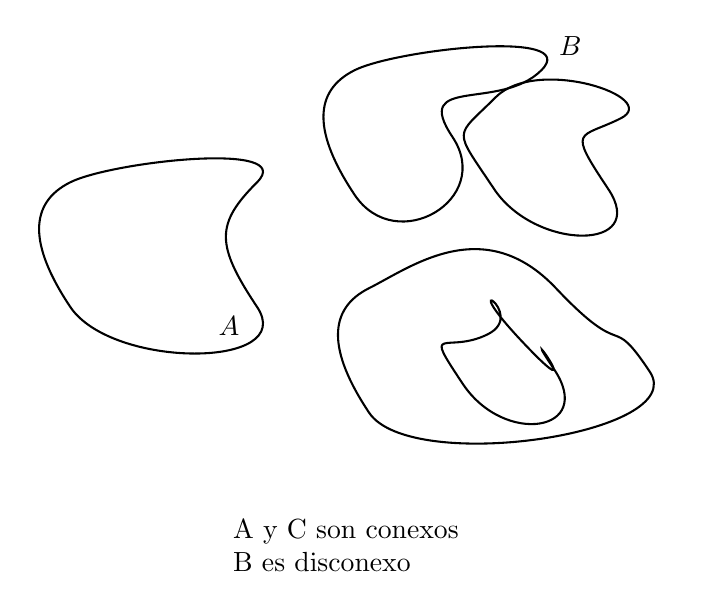
\begin{tikzpicture}[x=0.75pt,y=0.75pt,yscale=-1,xscale=1]
%uncomment if require: \path (0,300); %set diagram left start at 0, and has height of 300

%Shape: Polygon Curved [id:ds9079456360528385] 
\draw   (52,77) .. controls (72,67) and (162,57) .. (142,77) .. controls (122,97) and (122,107) .. (142,137) .. controls (162,167) and (72,167) .. (52,137) .. controls (32,107) and (32,87) .. (52,77) -- cycle ;
%Shape: Polygon Curved [id:ds9931025453530924] 
\draw   (189,23) .. controls (209,13) and (299,3) .. (279,23) .. controls (259,43) and (216.2,25.2) .. (236.2,55.2) .. controls (256.2,85.2) and (209,113) .. (189,83) .. controls (169,53) and (169,33) .. (189,23) -- cycle ;
%Shape: Polygon Curved [id:ds98969863279118] 
\draw   (317.2,46.2) .. controls (337.2,36.2) and (277,16) .. (257,36) .. controls (237,56) and (236.2,50.2) .. (256.2,80.2) .. controls (276.2,110.2) and (331.2,110.2) .. (311.2,80.2) .. controls (291.2,50.2) and (297.2,56.2) .. (317.2,46.2) -- cycle ;
%Shape: Polygon Curved [id:ds3993560047064726] 
\draw   (196,128) .. controls (216,118) and (251.2,91.2) .. (286,128) .. controls (320.8,164.8) and (311.2,138.2) .. (331.2,168.2) .. controls (351.2,198.2) and (216,218) .. (196,188) .. controls (176,158) and (176,138) .. (196,128) -- cycle ;
%Shape: Polygon Curved [id:ds4662727835448177] 
\draw   (253.2,150.2) .. controls (273.2,140.2) and (235.2,117.2) .. (270,154) .. controls (304.8,190.8) and (265.2,137.2) .. (285.2,167.2) .. controls (305.2,197.2) and (261.2,204.2) .. (241.2,174.2) .. controls (221.2,144.2) and (233.2,160.2) .. (253.2,150.2) -- cycle ;

% Text Node
\draw (129,237.9) node [anchor=north west][inner sep=0.75pt]   [align=left] {A y C son conexos \\B es disconexo};
% Text Node
\draw (122,140.1) node [anchor=north west][inner sep=0.75pt]    {$A$};
% Text Node
\draw (286,5.1) node [anchor=north west][inner sep=0.75pt]    {$B$};


\end{tikzpicture}
\end{center}
Un subconjunto $H$ del espacio métrico $M$ es \textbf{disconexo}, si existen abiertos $A$ y $B\ni A\cap H\neq \emptyset, B\cap H\neq \emptyset, (A\cap H)\cap (B\cap H)=\emptyset$ y $(A\cap H)\cup (B\cup H)=H$

\begin{center}
    

\tikzset{every picture/.style={line width=0.75pt}} %set default line width to 0.75pt        

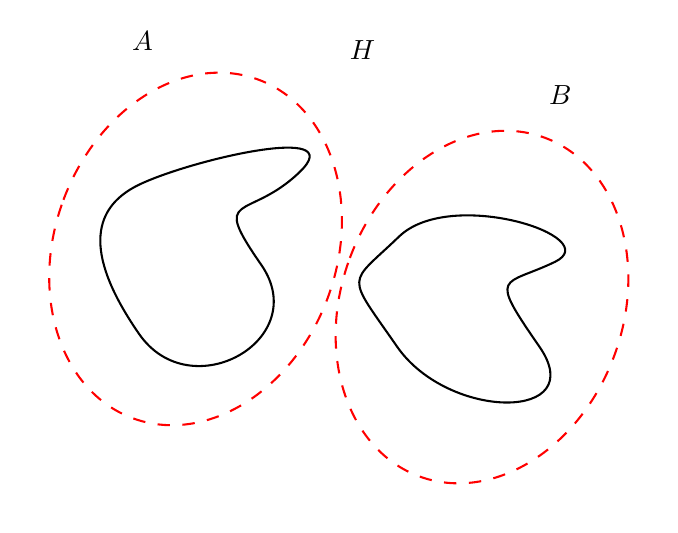
\begin{tikzpicture}[x=0.75pt,y=0.75pt,yscale=-1,xscale=1]
%uncomment if require: \path (0,300); %set diagram left start at 0, and has height of 300

%Shape: Polygon Curved [id:ds9931025453530924] 
\draw   (72.9,106.24) .. controls (97.83,94.25) and (175.13,76.22) .. (150.2,100.2) .. controls (125.27,124.18) and (106.81,108.87) .. (131.74,144.84) .. controls (156.67,180.81) and (97.83,214.14) .. (72.9,178.17) .. controls (47.97,142.2) and (47.97,118.22) .. (72.9,106.24) -- cycle ;
%Shape: Polygon Curved [id:ds98969863279118] 
\draw   (273.2,143.46) .. controls (298.13,131.47) and (223.08,107.25) .. (198.15,131.23) .. controls (173.22,155.21) and (172.22,148.26) .. (197.15,184.22) .. controls (222.08,220.19) and (290.65,220.19) .. (265.72,184.22) .. controls (240.78,148.26) and (248.26,155.45) .. (273.2,143.46) -- cycle ;
%Shape: Ellipse [id:dp5591846043661541] 
\draw  [color={rgb, 255:red, 255; green, 0; blue, 0 }  ,draw opacity=1 ][dash pattern={on 4.5pt off 4.5pt}] (36.46,113.52) .. controls (53.22,68.49) and (95.29,42.58) .. (130.44,55.66) .. controls (165.59,68.74) and (180.49,115.85) .. (163.74,160.88) .. controls (146.98,205.91) and (104.91,231.82) .. (69.76,218.74) .. controls (34.61,205.66) and (19.71,158.55) .. (36.46,113.52) -- cycle ;
%Shape: Ellipse [id:dp10167958292516732] 
\draw  [color={rgb, 255:red, 255; green, 0; blue, 0 }  ,draw opacity=1 ][dash pattern={on 4.5pt off 4.5pt}] (174.46,141.52) .. controls (191.22,96.49) and (233.29,70.58) .. (268.44,83.66) .. controls (303.59,96.74) and (318.49,143.85) .. (301.74,188.88) .. controls (284.98,233.91) and (242.91,259.82) .. (207.76,246.74) .. controls (172.61,233.66) and (157.71,186.55) .. (174.46,141.52) -- cycle ;

% Text Node
\draw (172.97,35.53) node [anchor=north west][inner sep=0.75pt]    {$H$};
% Text Node
\draw (68,31.1) node [anchor=north west][inner sep=0.75pt]    {$A$};
% Text Node
\draw (269,57.1) node [anchor=north west][inner sep=0.75pt]    {$B$};


\end{tikzpicture}
\end{center}
\end{definition}